% ====================================================
%  Astera Labs 调研汇报 — 组会 PPT
%  Author: 葛良晨
%  Date: 2026-05-21
%  Compile: latexmk -xelatex -shell-escape
% ====================================================
\documentclass[aspectratio=169, 10pt, UTF8]{ctexbeamer}

% ---------- 主题与颜色 ----------
\usetheme{Madrid}
\usecolortheme{default}

\definecolor{ieeeBlue}{RGB}{0, 83, 159}
\definecolor{ieeeRed}{RGB}{198, 38, 46}
\definecolor{ieeeGreen}{RGB}{0, 114, 41}
\definecolor{ieeeOrange}{RGB}{235, 110, 31}
\definecolor{darkGray}{RGB}{66, 66, 66}
\definecolor{gold}{RGB}{200, 150, 0}
\definecolor{darkblue}{RGB}{0, 0, 139}
\definecolor{darkgreen}{RGB}{0, 128, 0}
\definecolor{darkred}{RGB}{180, 0, 0}

\setbeamercolor{structure}{fg=ieeeBlue}
\setbeamercolor{alerted text}{fg=ieeeRed}
\setbeamercolor{example text}{fg=ieeeGreen}
\setbeamercolor{frametitle}{bg=ieeeBlue!15, fg=ieeeBlue}
\setbeamercolor{block title}{bg=ieeeBlue!15, fg=ieeeBlue}
\setbeamercolor{block body}{bg=ieeeBlue!5}
\setbeamercolor{block title example}{bg=ieeeGreen!15, fg=ieeeGreen}
\setbeamercolor{block body example}{bg=ieeeGreen!5}
\setbeamercolor{block title alerted}{bg=ieeeRed!15, fg=ieeeRed}
\setbeamercolor{block body alerted}{bg=ieeeRed!5}

% ---------- 包 ----------
\usepackage{graphicx}
\usepackage{booktabs}
\usepackage{tabularx}
\usepackage{multirow}
\usepackage[table]{xcolor}
\usepackage{amsmath,amssymb}
\usepackage{tikz}
\usetikzlibrary{positioning, calc, shapes.geometric, arrows.meta, backgrounds, fit}
\usepackage{hyperref}
\usepackage{twemojis}

% ---------- 自定义命令 ----------
\newcommand{\sourceT}[1]{{\small\textcolor{ieeeBlue}{[T#1]}}}
\newcommand{\unverified}{{\textcolor{ieeeRed}{\textbf{[未确认]}}}}
\newcommand{\speculation}{{\textcolor{ieeeOrange}{\textbf{[推测]}}}}
\newcommand{\marketing}{{\textcolor{ieeeOrange}{\textbf{[可能为营销]}}}}

% ---------- 页脚 ----------
\setbeamertemplate{footline}[frame number]

% ---------- 每节前显示目录 ----------
\AtBeginSection[]{
  \begin{frame}{本节内容}
    \tableofcontents[currentsection]
  \end{frame}
}

% ---------- 元信息 ----------
\title[Astera Labs 调研]{Astera Labs 全面调研汇报}
\subtitle{AI 基础设施连接芯片的工程与产业分析}
\author[葛良晨]{葛良晨}
\institute[组会汇报]{组会汇报 · 半导体行业分析}
\date{2026年5月21日}

\begin{document}

% ============================================
% \section{开场}
% ============================================

\begin{frame}
  \titlepage
\end{frame}

\begin{frame}{汇报大纲}
  \tableofcontents
\end{frame}

% ============================================
\section{公司概览与定位}
% ============================================

\begin{frame}{Astera Labs 基本信息}
  \begin{columns}[T]
    \begin{column}{0.55\textwidth}
      \begin{table}[]
        \begin{tabular}{ll}
          \toprule
          \textbf{属性} & \textbf{内容} \\
          \midrule
          成立 & 2017 年, Santa Clara, CA \\
          IPO & 2024 年 3 月, Nasdaq: ALAB \\
          IPO估值 & \$$\sim$5.5B, 募资 \$$\sim$713M \\
          商业模式 & Fabless (TSMC 代工) \\
          创始团队 & 3 位 TI 前员工 \\
          员工 & 未公开 \unverified{} \\
          FY2025 收入 & \textbf{\$852.5M} (+93\% YoY) \\
          毛利率 & \textbf{75-76\%} \\
          \bottomrule
        \end{tabular}
      \end{table}
    \end{column}
    \begin{column}{0.40\textwidth}
      \begin{block}{核心 Slogan}
        ``Purpose-Built Connectivity for Rack-Scale AI''
      \end{block}

      \begin{exampleblock}{产业链位置}
        Fabless 芯片设计 $\to$ TSMC 代工 $\to$ OSAT 封测 $\to$ Hyperscaler/Server OEM
      \end{exampleblock}

      \begin{alertblock}{关键事件}
        曾拒绝 Marvell 收购要约 \sourceT{3}
      \end{alertblock}
    \end{column}
  \end{columns}
\end{frame}

\begin{frame}{核心定位：三层架构}
  \centering
  \begin{tikzpicture}[
    node distance=0.2cm,
    layer/.style={rectangle, draw=ieeeBlue, fill=ieeeBlue!5, thick,
                  minimum width=7cm, minimum height=1.0cm, align=center,
                  rounded corners=4pt, font=\normalsize},
  ]
    \node[layer, fill=ieeeRed!8] (SLOGAN)
      {\textbf{``Purpose-Built Connectivity for Rack-Scale AI''}};
    \node[layer, fill=ieeeGreen!8, below=of SLOGAN] (POS)
      {定位：AI Infra 连接层供应商};
    \node[layer, fill=gold!15, below=of POS] (DIFF)
      {差异化：开放标准 (PCIe/CXL) vs 私有协议 (NVLink)};

    \node[layer, fill=ieeeBlue!12, below=0.5cm of DIFF] (L1)
      {\textbf{物理层}：Aries Retimer/Cable Module — 信号完整性};
    \node[layer, fill=ieeeBlue!8, below=0.3cm of L1] (L2)
      {\textbf{架构层}：Scorpio Fabric Switch — GPU/NIC/Storage 交换互连};
    \node[layer, fill=ieeeBlue!4, below=0.3cm of L2] (L3)
      {\textbf{系统层}：COSMOS — Telemetry \& Fleet Management};
  \end{tikzpicture}
\end{frame}

\begin{frame}{产业链位置}
  \centering
  \begin{tikzpicture}[
    node distance=0.8cm and 0.6cm,
    box/.style={rectangle, draw=ieeeBlue, thick, minimum width=2.2cm,
                minimum height=0.8cm, align=center, rounded corners=3pt,
                font=\footnotesize},
    highlight/.style={rectangle, draw=ieeeRed, fill=ieeeRed!10, thick,
                      minimum width=2.5cm, minimum height=0.8cm, align=center,
                      rounded corners=3pt, font=\footnotesize},
    arrow/.style={->, >=Stealth, thick}
  ]
    % Top row: upstream
    \node[box, fill=gray!10] (EDA) {EDA/IP\\Synopsys/Cadence};
    \node[box, fill=gray!10, right=of EDA] (FAB) {晶圆代工\\TSMC};
    \node[box, fill=gray!10, right=of FAB] (OSAT) {封装测试\\OSAT};

    % Center: Astera Labs
    \node[highlight, below=of FAB] (AST) {\textbf{Astera Labs}\\\textbf{Fabless Designer}};

    % Bottom: product lines
    \node[box, fill=ieeeBlue!5, below left=of AST] (P1) {Scorpio\\Fabric Switch};
    \node[box, fill=ieeeBlue!5, below=of AST] (P2) {Aries\\Retimer/Cable};
    \node[box, fill=ieeeBlue!5, below right=of AST] (P3) {Leo/Taurus\\CXL/Ethernet};

    % Customers
    \node[box, fill=ieeeGreen!10, below=of P2, minimum width=3.0cm] (CUST)
      {Hyperscalers\\+ Server OEM\\+ GPU Vendor};

    \draw[arrow] (EDA) -- (AST);
    \draw[arrow] (FAB) -- (AST);
    \draw[arrow] (OSAT) -- (AST);
    \draw[arrow] (AST) -- (P1);
    \draw[arrow] (AST) -- (P2);
    \draw[arrow] (AST) -- (P3);
    \draw[arrow] (P1) -- (CUST);
    \draw[arrow] (P2) -- (CUST);
    \draw[arrow] (P3) -- (CUST);
  \end{tikzpicture}
\end{frame}

\begin{frame}{Rack-Scale AI 与连接需求}
  \centering
  \begin{tikzpicture}[
    scale=0.82,
    rack/.style={rectangle, draw=ieeeBlue, fill=ieeeBlue!3, thick,
                 minimum width=2.8cm, minimum height=3.5cm, rounded corners=3pt},
    gpu/.style={rectangle, draw=ieeeRed, fill=ieeeRed!8, thick,
                minimum width=1.0cm, minimum height=0.55cm, align=center,
                font=\tiny, rounded corners=1pt},
    scorp/.style={rectangle, draw=gold, fill=yellow!10, thick,
                  minimum width=1.05cm, minimum height=0.5cm, align=center,
                  font=\tiny, rounded corners=2pt},
    connect/.style={-, thick, ieeeBlue!70},
    soArrow/.style={->, >=Stealth, very thick, ieeeGreen!65},
  ]
    % Rack 1
    \node[rack] (R1) {};
    \node[font=\footnotesize\bfseries, above=0.1cm of R1.north] {Rack 1 (Scale-Up)};

    \foreach \x/\y/\name in {-0.68/1.1/G1, 0.68/1.1/G2, -0.68/0.35/G3, 0.68/0.35/G4, -0.68/-0.4/G5, 0.68/-0.4/G6} {
      \node[gpu] (\name) at ($(R1.center)+(\x,\y)$) {GPU};
    }
    \node[scorp] (S1) at ($(R1.center)+(0,-1.15)$) {Scorpio};
    \foreach \i in {1,...,6} { \draw[connect] (G\i) -- (S1); }

    % Logical "Big GPU"
    \draw[draw=ieeeRed, densely dashed, very thick, rounded corners=4pt]
      ($(R1.north west)+(-0.12,0.2)$) rectangle ($(R1.south east)+(0.12,-0.05)$);
    \node[font=\footnotesize\bfseries, ieeeRed, above=0.5cm of R1.north] {Logical ``Big GPU''};

    % Rack 2
    \node[rack, right=2.5cm of R1] (R2) {};
    \node[font=\footnotesize\bfseries, above=0.1cm of R2.north] {Rack N};
    \foreach \x/\y/\name in {-0.68/0.45/G7, 0.68/0.45/G8, -0.68/-0.3/G9, 0.68/-0.3/G10} {
      \node[gpu] (\name) at ($(R2.center)+(\x,\y)$) {GPU};
    }
    \node[scorp] (S2) at ($(R2.center)+(0,-1.15)$) {Scorpio};
    \foreach \i in {7,...,10} { \draw[connect] (G\i) -- (S2); }

    % Scale-Out Network
    \node[rectangle, draw=ieeeGreen, fill=ieeeGreen!5, thick,
          minimum width=9cm, minimum height=0.45cm, align=center,
          font=\footnotesize, rounded corners=2pt]
          (SONET) at ($(R1.south)!0.5!(R2.south)+(0,-0.65cm)$)
          {Scale-Out Network (InfiniBand / Ethernet) — 100m+};

    \draw[soArrow] (S1.south) -- (S1.south |- SONET.north);
    \draw[soArrow] (S2.south) -- (S2.south |- SONET.north);

    \node[font=\footnotesize, text width=10cm, align=center, below=0.3cm of SONET]
      {单机架 GPU 通过 Scorpio 形成逻辑大 GPU (Scale-Up)；跨机架走 Ethernet/IB (Scale-Out)};
  \end{tikzpicture}
\end{frame}

\begin{frame}{Scale-Up Fabric vs Scale-Out Network}
  \centering
  \begin{tikzpicture}[
    scale=0.55,
    title/.style={font=\bfseries\small},
    nodebox/.style={rectangle, draw=ieeeBlue, fill=ieeeBlue!5, thick,
                    minimum width=1.6cm, minimum height=0.65cm, align=center,
                    font=\footnotesize, rounded corners=2pt},
    gpubox/.style={rectangle, draw=ieeeRed, fill=ieeeRed!8, thick,
                   minimum width=1.0cm, minimum height=0.65cm, align=center,
                   font=\footnotesize},
    arrow/.style={->, >=Stealth, thick},
    bidir/.style={<->, >=Stealth, thick},
    bgbox/.style={rounded corners, thick, inner sep=8pt},
  ]
    % Scale-Up Zone
    \node[title, ieeeRed] (SU_LABEL) {Scale-Up Fabric (机架内, <10m, 超高带宽/超低延迟)};
    \node[font=\footnotesize\color{ieeeRed}, below=0.1cm of SU_LABEL] (SU_EX)
      {例: NVLink 900\,GB/s per GPU, Scorpio X-Series};

    \node[gpubox, below=0.3cm of SU_EX] (SU2) {GPU 1};
    \node[gpubox, left=of SU2] (SU1) {GPU 0};
    \node[gpubox, right=of SU2] (SU3) {GPU N};

    \node[rectangle, draw=gold, fill=yellow!10, thick,
          minimum width=2.2cm, minimum height=0.6cm, align=center,
          font=\footnotesize, below=0.3cm of SU2] (SW) {Scorpio X-Series};

    \node[nodebox, fill=ieeeGreen!8, left=0.6cm of SW] (SU_MEM) {CXL Memory\\Pool};
    \node[nodebox, fill=ieeeGreen!8, right=0.6cm of SW] (SU_NIC) {NIC};

    \draw[bidir, ieeeRed] (SU1) -- (SW);
    \draw[bidir, ieeeRed] (SU2) -- (SW);
    \draw[bidir, ieeeRed] (SU3) -- (SW);
    \draw[arrow, ieeeBlue] (SW) -- (SU_MEM);
    \draw[arrow, ieeeBlue] (SW) -- (SU_NIC);

    \begin{scope}[on background layer]
      \node[bgbox, fill=ieeeRed!3, draw=ieeeRed,
            fit=(SU_LABEL)(SU_EX)(SU3)(SW)(SU_MEM)] (SU_BG) {};
    \end{scope}

    % Astera connector
    \node[rectangle, draw=gold, fill=yellow!15, thick,
          minimum width=2.0cm, minimum height=0.6cm, align=center,
          font=\footnotesize\bfseries, below=0.4cm of SW] (AST_POS)
          {Astera Labs\\交汇点};

    % Scale-Out Zone
    \node[rectangle, draw=ieeeGreen, fill=ieeeGreen!5, thick,
          minimum width=2.8cm, minimum height=0.5cm, align=center,
          font=\footnotesize, below=0.4cm of AST_POS] (ENET)
          {Ethernet / IB Switch Fabric};

    \node[nodebox, fill=ieeeBlue!5, below=0.3cm of ENET] (NODE2) {Compute\\Node 1};
    \node[nodebox, fill=ieeeBlue!5, left=of NODE2] (NODE1) {Compute\\Node 0};
    \node[nodebox, fill=ieeeBlue!5, right=of NODE2] (NODE3) {Compute\\Node N};

    \draw[arrow, ieeeGreen] (NODE1) -- (ENET);
    \draw[arrow, ieeeGreen] (NODE2) -- (ENET);
    \draw[arrow, ieeeGreen] (NODE3) -- (ENET);

    \node[font=\footnotesize\color{ieeeGreen}, below=0.1cm of NODE2] (SO_EX)
      {例: InfiniBand 400\,GB/s, Ethernet 800G};
    \node[title, ieeeGreen, below=0.1cm of SO_EX] (SO_LABEL)
      {Scale-Out Network (跨机架, 100m+, 可扩展性)};

    \begin{scope}[on background layer]
      \node[bgbox, fill=ieeeGreen!3, draw=ieeeGreen,
            fit=(ENET)(NODE3)(SO_LABEL)] (SO_BG) {};
    \end{scope}

    % Connector arrows
    \draw[arrow, ieeeBlue, very thick] (AST_POS.north) -- (SW.south);
    \draw[arrow, ieeeGreen, very thick] (AST_POS.south) -- (ENET.north);
    \node[font=\footnotesize, text width=1.8cm, align=center,
          right=0.2cm of AST_POS] {Aries\\Cable};
  \end{tikzpicture}
\end{frame}

\begin{frame}{为什么 Hyperscaler 需要独立连接供应商}
  \begin{enumerate}
    \item \textbf{避免 NVIDIA 锁定}
    \begin{itemize}
      \item NVLink/NVSwitch 仅 NVIDIA GPU 可用
      \item Hyperscaler 需要 PCIe/CXL 开放标准维持多 GPU 供应商策略
    \end{itemize}

    \item \textbf{统一管理平面}
    \begin{itemize}
      \item GPU/NIC/NVMe 连接分散在不同供应商 → 运维灾难
    \end{itemize}

    \item \textbf{定制化需求}
    \begin{itemize}
      \item Hyperscaler 需要定制拓扑，Broadcom 等大厂未必愿意配合
    \end{itemize}

    \item \textbf{信号完整性挑战}
    \begin{itemize}
      \item PCIe 6 PAM4 时代，SI 挑战指数增长
    \end{itemize}

    \item \textbf{供应链安全}
    \begin{itemize}
      \item 任何关键组件至少需要 2 个来源 (second source)
    \end{itemize}
  \end{enumerate}
\end{frame}

% ============================================
\section{产品线全景}
% ============================================

\begin{frame}{全产品线总览}
  \begin{table}[h]
    \centering
    \small
    \begin{tabular}{lllp{0.30\textwidth}}
      \toprule
      \textbf{产品} & \textbf{类型} & \textbf{协议/标准} & \textbf{核心价值} \\
      \midrule
      \rowcolor{ieeeBlue!12}
      Scorpio X & Smart Fabric Switch & Memory Semantic & GPU Scale-Up, 320 lanes \\
      \rowcolor{ieeeBlue!8}
      Scorpio P & Smart Fabric Switch & PCIe 6 & PCIe Fabric, 32–320 lanes \\
      \midrule
      \rowcolor{ieeeGreen!10}
      Aries Retimer & Smart DSP Retimer & PCIe 6 / CXL 3.x & 信号再生, DSP 均衡 \\
      \rowcolor{ieeeGreen!10}
      Aries Smart Cable & Active Cable Module & PCIe 6 / CXL 3.x & 7m 铜缆, 64 GT/s \\
      \rowcolor{ieeeGreen!10}
      Aries Gearbox & Protocol Bridge & PCIe 6 $\leftrightarrow$ 5 & 代际过渡 \\
      \midrule
      Leo & CXL Memory Ctrl & CXL 1.1 & DDR5 内存扩展/池化 \\
      Taurus & Active Cable Module & Ethernet & 800G per link, 7m \\
      \midrule
      \rowcolor{ieeeOrange!15}
      COSMOS & Software Platform & — & Telemetry, Fleet Mgmt, RAS \\
      \bottomrule
    \end{tabular}
  \end{table}
\end{frame}

\begin{frame}{产品拓扑与战略关系}
  \centering
  \begin{figure}[htb]
    \centering
    \begin{tikzpicture}[
        node distance=0.4cm and 0.6cm,
        product/.style={rectangle, draw=darkblue, fill=blue!5, thick, minimum width=2.2cm, minimum height=0.8cm, align=center, rounded corners=3pt},
        platform/.style={rectangle, draw=darkgreen, fill=green!10, thick, minimum width=5.5cm, minimum height=0.8cm, align=center, rounded corners=3pt},
        arrow/.style={->, >=Stealth, thick, darkblue},
        arrow_sw/.style={->, >=Stealth, thick, darkgreen}
    ]
        % 第一行：Aries 产品
        \node[product] (ARIES_R) {Aries Retimer\\(SI 信号再生)};
        \node[product, right= 4cm of ARIES_R] (ARIES_G) {Aries Gearbox\\(PCIe 5$\leftrightarrow$6桥接)};

        % 第二行：居中于 ARIES_R 与 ARIES_G 之间
        \node[product, below=1cm] (ARIES_C) at ($(ARIES_R)!0.5!(ARIES_G)$) {Aries Smart Cable\\(智能有源电缆)};

        % 第三行：Scorpio 系列，位于 ARIES_C 下方两侧
        \node[product, below left= of ARIES_C] (SCORPIO_P) {Scorpio P-Series\\(PCIe 6 Fabric Switch)};
        \node[product, fill=darkred!15, below right= of ARIES_C] (SCORPIO_X) {Scorpio X-Series\\(Memory Semantic Fabric)};

        % 第四行：COSMOS 居中于 Scorpio 节点之间
        \node[platform, minimum width=5cm, below=1.5cm] (COSMOS) at ($(SCORPIO_P)!0.5!(SCORPIO_X)$) {COSMOS 软件平台 (统一管理)};

        % 第五行：Leo 与 Taurus 位于 COSMOS 下方两侧
        \node[product, below left= of COSMOS] (LEO) {Leo\\(CXL Memory Ctrl)};
        \node[product, below right= of COSMOS] (TAURUS) {Taurus\\(Ethernet Cable)};

        \draw[arrow_sw] (ARIES_R) -- (COSMOS);
        \draw[arrow_sw] (ARIES_C) -- (COSMOS);
        \draw[arrow_sw] (ARIES_G) -- (COSMOS);
        \draw[arrow_sw] (SCORPIO_P) -- (COSMOS);
        \draw[arrow_sw] (SCORPIO_X) -- (COSMOS);
        \draw[arrow_sw] (LEO) -- (COSMOS);
        \draw[arrow_sw] (TAURUS) -- (COSMOS);

        \draw[arrow, dashed, darkred] (ARIES_R) -- node[midway, left, font=\footnotesize] {DSP核心} (ARIES_C);
        \draw[arrow, dashed, darkred] (SCORPIO_P) -- node[midway, right, font=\footnotesize] {Scale-Up} (SCORPIO_X);
    \end{tikzpicture}
    \caption{产品拓扑关系图}
    \label{fig:product-topology}
\end{figure}
\end{frame}

\begin{frame}{产品在 AI 数据中心中的物理位置}
  \centering
  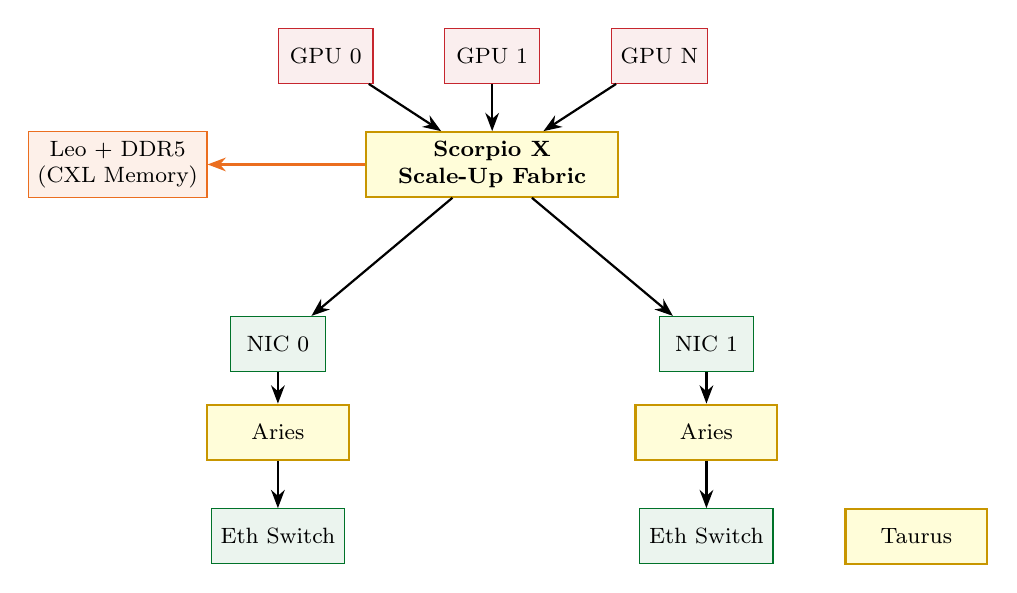
\begin{tikzpicture}[
    node distance=0.7cm and 0.9cm,
    gpu/.style={rectangle, draw=ieeeRed, fill=ieeeRed!8, minimum width=1.2cm,
                minimum height=0.7cm, align=center, font=\footnotesize},
    ast/.style={rectangle, draw=gold, fill=yellow!15, thick, minimum width=1.8cm,
                minimum height=0.7cm, align=center, font=\footnotesize\bfseries},
    dev/.style={rectangle, draw=ieeeGreen, fill=ieeeGreen!8, minimum width=1.2cm,
                minimum height=0.7cm, align=center, font=\footnotesize},
    arrow/.style={->, >=Stealth, thick},
  ]
    % GPU row
    \node[gpu] (GPU1) {GPU 0};
    \node[gpu, right=of GPU1] (GPU2) {GPU 1};
    \node[gpu, right=of GPU2] (GPU3) {GPU N};

    % Scorpio
    \node[ast, below=0.6cm of GPU2, minimum width=3.2cm] (SCORP) {Scorpio X\\Scale-Up Fabric};

    % NICs
    \node[dev, below left=1.5cm and 0.5cm of SCORP] (NIC1) {NIC 0};
    \node[dev, below right=1.5cm and 0.5cm of SCORP] (NIC2) {NIC 1};

    % Aries + Ethernet
    \node[ast, font=\footnotesize, below=0.4cm of NIC1] (ARIES1) {Aries};
    \node[ast, font=\footnotesize, below=0.4cm of NIC2] (ARIES2) {Aries};
    \node[dev, below=0.6cm of ARIES1] (SW1) {Eth Switch};
    \node[dev, below=0.6cm of ARIES2] (SW2) {Eth Switch};
    \node[ast, font=\footnotesize, right=of SW2] (TAURUS_N) {Taurus};

    % Leo
    \node[dev, draw=ieeeOrange, fill=ieeeOrange!10, minimum width=2.0cm,
          minimum height=0.7cm, align=center, font=\footnotesize,
          left=2.0cm of SCORP] (LEO_N) {Leo + DDR5\\(CXL Memory)};

    \draw[arrow] (GPU1) -- (SCORP);
    \draw[arrow] (GPU2) -- (SCORP);
    \draw[arrow] (GPU3) -- (SCORP);
    \draw[arrow] (SCORP) -- (NIC1);
    \draw[arrow] (SCORP) -- (NIC2);
    \draw[arrow] (NIC1) -- (ARIES1);
    \draw[arrow] (NIC2) -- (ARIES2);
    \draw[arrow] (ARIES1) -- (SW1);
    \draw[arrow] (ARIES2) -- (SW2);
    \draw[arrow, ieeeOrange, thick] (SCORP) -- (LEO_N);
  \end{tikzpicture}
\end{frame}

\begin{frame}{Astera Labs 产品在数据中心中的物理位置}
  \begin{center}
    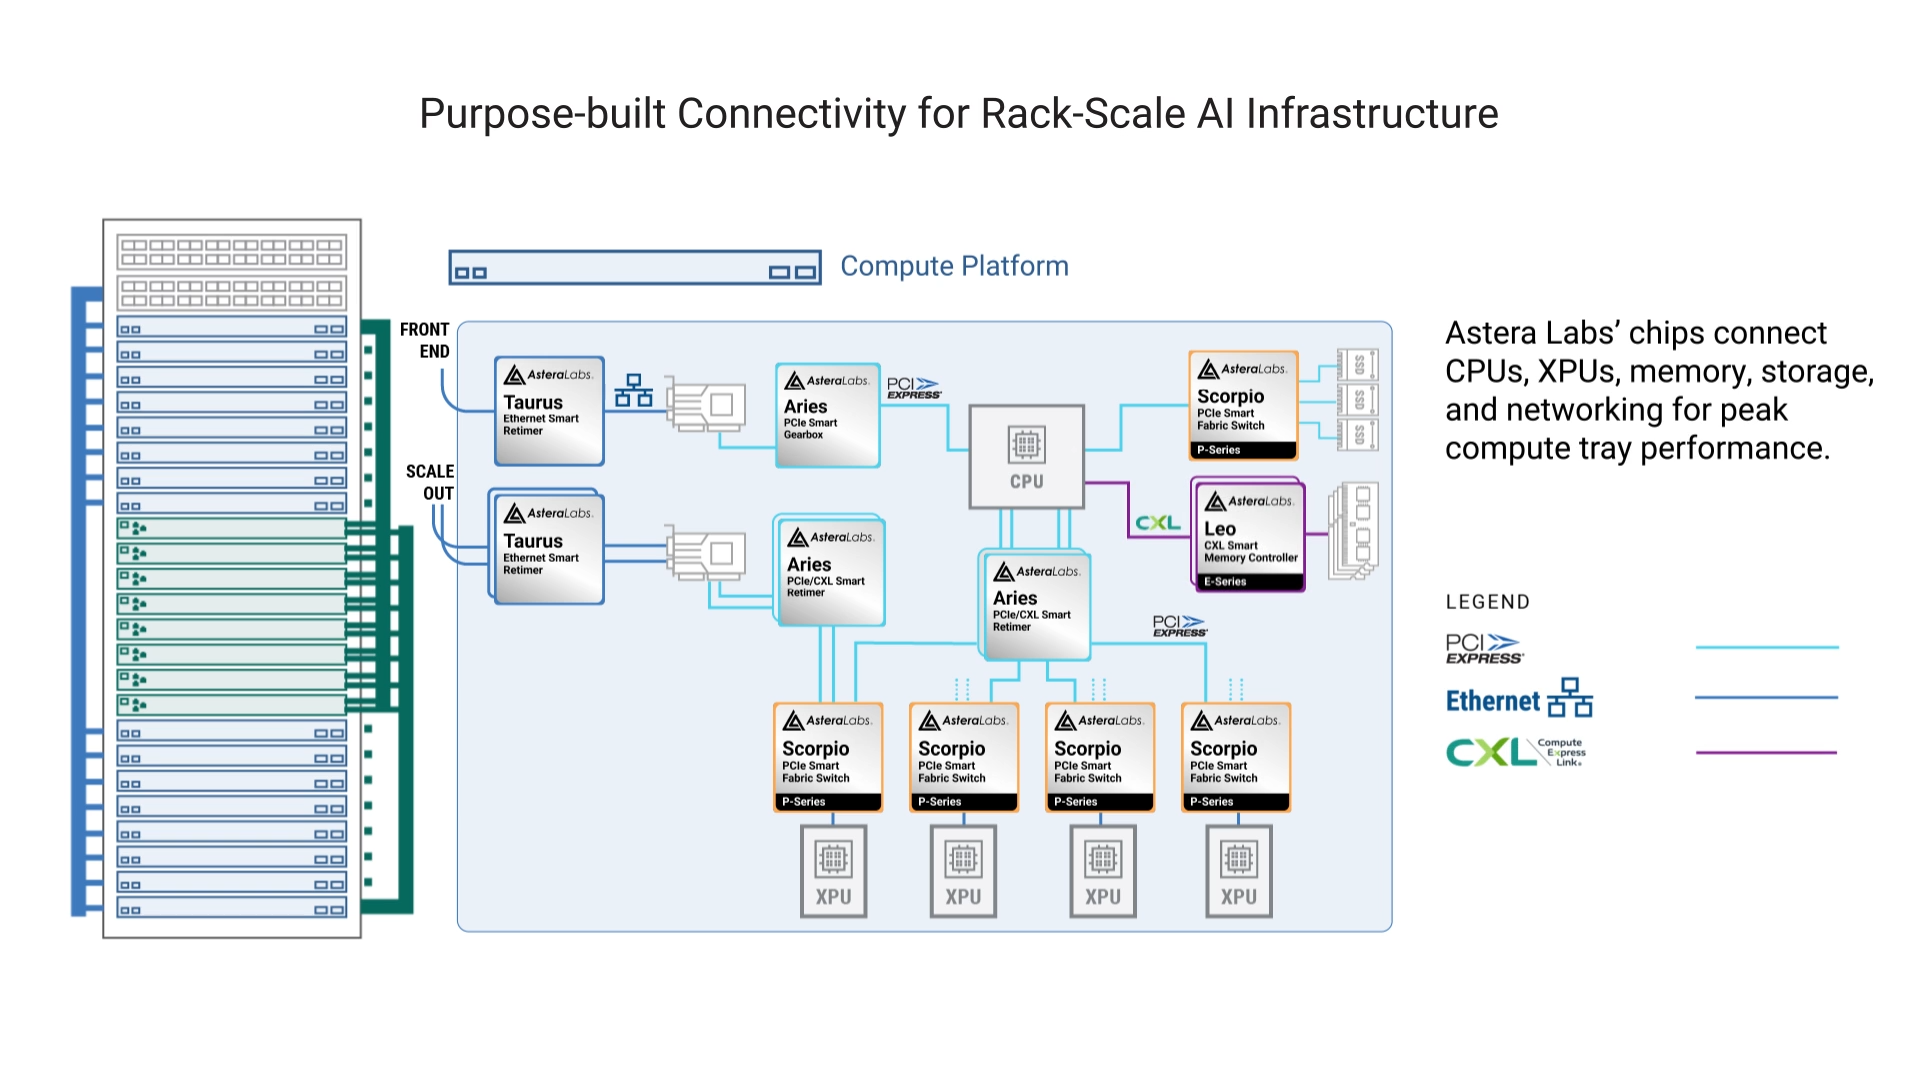
\includegraphics[width=0.9\textwidth]{assets/location.png}
  \end{center}
\end{frame}

% ============================================
\begin{frame}{PCIe 树形拓扑 $\to$ PCIe Fabric $\to$ CXL Fabric}
  \centering
  \begin{tikzpicture}[
    scale=0.75,
    node distance=0.2cm and 0.6cm,
    title/.style={font=\bfseries\footnotesize},
    cpu/.style={rectangle, draw=ieeeBlue, fill=ieeeBlue!8, thick,
                minimum width=1.2cm, minimum height=0.7cm, align=center,
                font=\footnotesize},
    dev/.style={rectangle, draw=ieeeRed, fill=ieeeRed!6, thick,
                minimum width=1.2cm, minimum height=0.7cm, align=center,
                font=\footnotesize},
    mem/.style={rectangle, draw=ieeeGreen, fill=ieeeGreen!8, thick,
                minimum width=1.2cm, minimum height=0.7cm, align=center,
                font=\footnotesize},
    sw/.style={rectangle, draw=gold, fill=yellow!12, thick,
               minimum width=1.4cm, minimum height=0.7cm, align=center,
               font=\footnotesize},
    arrow/.style={->, >=Stealth, thick},
    bidir/.style={<->, >=Stealth, thick},
    note/.style={font=\footnotesize\color{darkGray}, align=center},
  ]
    % Column 1: Traditional PCIe Tree
    \node[title, ieeeBlue] (T1) {传统 PCIe 树形拓扑};
    \node[cpu, below=0.3cm of T1] (CPU1) {CPU\\Root};
    \node[dev, below=0.5cm of CPU1] (D2) {NVMe};
    \node[dev, left=of D2]  (D1) {GPU};
    \node[dev, right=of D2] (D3) {NIC};
    \draw[arrow] (CPU1) -- (D1);
    \draw[arrow] (CPU1) -- (D2);
    \draw[arrow] (CPU1) -- (D3);
    \draw[draw=ieeeRed, dashed] (D1) to[bend left=22]
      node[midway, above, font=\tiny\bfseries, ieeeRed] {$\times$ 不可直连} (D3);
    \node[note, below=0.25cm of D2, text width=2.8cm] (N1)
      {单一根节点\\设备间无法直连};

    % Column 2: PCIe Fabric
    \node[title, ieeeBlue, right=1.8cm of T1] (T2) {PCIe Fabric (Scorpio)};
    \node[sw, below=0.3cm of T2] (SW1) {Scorpio\\Switch};
    \node[dev, below=0.5cm of SW1] (F2) {GPU};
    \node[dev, left=of F2]  (F1) {GPU};
    \node[dev, right=of F2] (F3) {GPU};
    \node[dev, below=0.4cm of F2] (F5) {NVMe};
    \node[dev, left=of F5]  (F4) {NIC};
    \node[dev, right=of F5] (F6) {NIC};
    \draw[arrow] (SW1) -- (F1);
    \draw[arrow] (SW1) -- (F2);
    \draw[arrow] (SW1) -- (F3);
    \draw[arrow] (SW1) -- (F4);
    \draw[arrow] (SW1) -- (F5);
    \draw[arrow] (SW1) -- (F6);
    \draw[bidir, ieeeRed] (F1) -- (F2);
    \draw[bidir, ieeeRed] (F2) -- (F3);
    \node[note, below=0.25cm of F5, text width=2.8cm] (N2)
      {任意设备互连\\Mesh/Torus 拓扑};

    % Column 3: CXL Fabric
    \node[title, ieeeBlue, right=1.8cm of T2] (T3) {CXL Fabric (Memory Semantic)};
    \node[sw, below=0.3cm of T3] (SW2) {CXL\\Switch};
    \node[cpu, below left=0.5cm and 0.5cm of SW2] (C1) {CPU};
    \node[dev, below right=0.5cm and 0.5cm of SW2] (C2) {GPU};
    \node[mem, below=0.4cm of C1] (M1) {DDR5\\Pool};
    \node[mem, below=0.4cm of C2] (M2) {DDR5\\Pool};
    \draw[arrow] (SW2) -- (C1);
    \draw[arrow] (SW2) -- (C2);
    \draw[arrow] (SW2) -- (M1);
    \draw[arrow] (SW2) -- (M2);
    \draw[draw=ieeeGreen, densely dashed, thick] (C1) to[bend right=25]
      node[midway, right, font=\tiny\bfseries, ieeeGreen] {cache coherent} (M1);
    \node[note, below=0.25cm of M1, text width=3.2cm] (N3)
      {CPU/GPU 直接 load/store\\访问远端内存};

    % Dividers
    \coordinate (DX1) at ($(T1.east)!0.5!(T2.west)$);
    \coordinate (DX2) at ($(T2.east)!0.5!(T3.west)$);
    \draw[dashed, gray!50, thick] ($(DX1)+(0,0.2)$) -- ($(DX1 |- N2.south)+(0,-0.4)$);
    \draw[dashed, gray!50, thick] ($(DX2)+(0,0.2)$) -- ($(DX2 |- N2.south)+(0,-0.4)$);

    % Legend
    \node[rectangle, draw=gray!40, fill=gray!3, rounded corners=2pt,
          text width=0.92\linewidth, align=center, font=\footnotesize,
          inner sep=5pt, below=0.8cm of N2] {
      \textbf{关键区别}：传统 PCIe 中 GPU 不可直连（须经 CPU）；
      PCIe Fabric (Scorpio) 允许任意设备直连，支持灵活 Mesh 拓扑；
      CXL Fabric 进一步支持 cache-coherent 的 load/store 内存访问语义。};
  \end{tikzpicture}
\end{frame}

\section{Scorpio: 核心产品深度分析}
% ============================================

\begin{frame}{Scorpio 是什么？}
  \begin{alertblock}{核心定义}
    不是传统 PCIe Switch，不是 NVSwitch 复制品。\\
    \textbf{新型 Smart Fabric Switch} — 基于 PCIe 6 PHY (64 GT/s PAM4)，运行多种协议。
  \end{alertblock}

  \begin{table}[h]
    \centering
    \begin{tabular}{lcc}
      \toprule
      \textbf{特性} & \textbf{Scorpio X-Series} & \textbf{Scorpio P-Series} \\
      \midrule
      定位 & Memory Semantic AI Fabric & PCIe 6 Fabric Switch \\
      Lane Count & \textbf{320 lanes} (业界最大) & 32–320 lanes \\
      协议 & Memory Semantic + Custom & PCIe 6 / CXL 3.x \\
      目标应用 & GPU Scale-Up Fabric & 通用 I/O Fabric \\
      HW Collective Ops & Hypercast (All-Reduce 等) & — \\
      出货状态 & 已出货至 Leading Hyperscalers & 已 Demo (H200+ConnectX-8) \\
      \bottomrule
    \end{tabular}
  \end{table}
\end{frame}

\begin{frame}{Scorpio 技术架构分层}
  \centering
  \begin{tikzpicture}[
    node distance=0.2cm,
    layer/.style={rectangle, draw=ieeeBlue, fill=ieeeBlue!5, thick,
                  minimum width=8cm, minimum height=0.85cm, align=center,
                  rounded corners=3pt, font=\normalsize},
  ]
    \node[layer, fill=ieeeRed!10] (L5) {\textbf{管理层}：Fabric Manager via COSMOS Integration};
    \node[layer, fill=ieeeOrange!10, below=of L5] (L4) {\textbf{加速层}：HW-Accelerated Collective Ops (Hypercast)};
    \node[layer, fill=gold!15, below=of L4] (L3) {\textbf{协议引擎}：PCIe 6 FLIT + Memory Semantic Protocol Engine};
    \node[layer, fill=ieeeGreen!8, below=of L3] (L2) {\textbf{交换层}：High-Radix Crossbar Switch Fabric};
    \node[layer, fill=ieeeBlue!12, below=of L2] (L1) {\textbf{物理层}：320$\times$ SerDes @ 64 GT/s PAM4};

    \node[font=\footnotesize, text width=8cm, align=left, below=0.6cm of L1] {
      \textbf{已确认} \sourceT{2}：320 lane, 64 GT/s, high-radix single-hop, Hypercast, per-port telemetry \\
      \textbf{未公开} \unverified{}：端到端延迟(ns)、功耗(W)、die size、制程节点
    };
  \end{tikzpicture}
\end{frame}

\begin{frame}{为什么 AI GPU 集群需要 Scorpio}
  \begin{enumerate}
    \item \textbf{GPU Scale-Up Fabric}
    \begin{itemize}
      \item NVSwitch 仅支持 NVIDIA GPU
      \item 异构集群 (AMD/Intel/自研 ASIC) 需要开放互连方案
    \end{itemize}

    \item \textbf{GPU-to-NIC-to-Storage 直通}
    \begin{itemize}
      \item 消除 CPU bottleneck — 数据路径 GPU $\to$ NIC 不经 CPU
    \end{itemize}

    \item \textbf{MoE 模型通信优化}
    \begin{itemize}
      \item Mixture-of-Experts：稀疏但大带宽的 all-to-all 通信
      \item Hypercast：交换机内部聚合数据 (All-Reduce 求和)，减少网络流量
    \end{itemize}

    \item \textbf{CXL 内存池}
    \begin{itemize}
      \item GPU 通过 Scorpio 访问 CXL-attached DDR5，扩展 KV Cache 容量
    \end{itemize}
  \end{enumerate}
\end{frame}

\begin{frame}{Scorpio vs NVSwitch 深度对比}
  \begin{table}[h]
    \centering
    \begin{tabular}{lcc}
      \toprule
      \textbf{对比维度} & \textbf{Scorpio X-Series} & \textbf{NVIDIA NVSwitch (H100)} \\
      \midrule
      物理层 & PCIe 6 (64 GT/s PAM4) & NVLink 4 (100 GT/s) \\
      Per-GPU 带宽 & $\sim$128 GB/s (x16) & \textbf{900 GB/s} (18 links) \\
      协议 & \textbf{开放 PCIe/CXL + Custom} & 私有 NVLink \\
      GPU 兼容 & \textbf{任何 PCIe 设备} & 仅 NVIDIA GPU \\
      Radix & \textbf{320 lanes} & 连接 8 GPU (可级联) \\
      Collective Ops & Hypercast (in-fabric) & SHARP (in-network) \\
      软件 & COSMOS (跨厂商) & NVSwitch Fabric Manager \\
      \bottomrule
    \end{tabular}
  \end{table}

  \begin{exampleblock}{核心差异}
    绝对带宽差距 $\sim$7$\times$，但 Scorpio 的价值在于\textbf{开放性与异构兼容性}。
    非 NVIDIA GPU 的 PCIe 侧即使 H200 也仅 x16 PCIe 5 (64 GB/s) —— Scorpio 匹配了这个能力。
  \end{exampleblock}
\end{frame}

\begin{frame}{Scorpio vs Broadcom PEX}
  \begin{table}[h]
    \centering
    \begin{tabular}{lcc}
      \toprule
      \textbf{维度} & \textbf{Scorpio (Astera)} & \textbf{PEX 系列 (Broadcom)} \\
      \midrule
      PCIe 世代 & \textbf{PCIe 6} & PCIe 5 为主, 6 roadmapped \\
      最大 lane & \textbf{320} & $\sim$144 (公开) \\
      Memory Semantic & \textbf{支持} & 标准 PCIe only \\
      HW Collective Ops & \textbf{支持 (Hypercast)} & 未知 \\
      AI 优化 & \textbf{从零为 AI 设计} & 通用数据中心 \\
      COSMOS & \textbf{原生集成} & 无等效平台 \\
      市场成熟度 & 新进入者 & 极成熟 (十多年积累) \\
      \bottomrule
    \end{tabular}
  \end{table}

  \begin{alertblock}{威胁评估：中等}
    Scorpio 主要威胁 \textbf{AI-specific 增量市场}，非 Broadcom 传统企业/存储 switch。
    但 PCIe 6 是新赛道 — 所有人同一起跑线。
  \end{alertblock}
\end{frame}

% ============================================
\section{Aries: 信号完整性基石}
% ============================================

\begin{frame}{Retimer 基础知识}
  \centering
  \begin{tikzpicture}[
    node distance=0.5cm,
    block/.style={rectangle, draw=ieeeBlue, fill=ieeeBlue!5, thick,
                  minimum width=1.8cm, minimum height=0.8cm, align=center,
                  rounded corners=3pt},
    signal/.style={->, >=Stealth, thick},
  ]
    \node[block] (TX) {TX\\发送端};
    \node[block, right=of TX] (CH) {Channel\\PCB/背板};
    \node[block, right=of CH, fill=ieeeRed!10] (RT) {Retimer\\CDR+再生};
    \node[block, right=of RT] (CH2) {Channel};
    \node[block, right=of CH2] (RX) {RX\\接收端};

    \draw[signal] (TX) -- (CH);
    \draw[signal, ieeeRed, very thick] (CH) -- (RT)
      node[midway, above, font=\tiny] {弱信号};
    \draw[signal, ieeeGreen, very thick] (RT) -- (CH2)
      node[midway, above, font=\tiny] {干净信号};
    \draw[signal] (CH2) -- (RX);
  \end{tikzpicture}

  \vspace{6pt}
  \begin{table}[h]
    \centering
    \tiny
    \begin{tabular}{lccc}
      \toprule
      \textbf{} & \textbf{Redriver} & \textbf{Ana Retimer} & \textbf{DSP Retimer} \\
      \midrule
      时钟恢复 & 无 & 有 & 有 \\
      延迟 & $<$100ps & 10-20ns & 20-50ns \\
      噪声 & \textbf{放大} & 消除 & \textbf{完全消除} \\
      PCIe 6 & \textbf{不可用} & 勉强 & \textbf{必需} \\
      \bottomrule
    \end{tabular}
  \end{table}

  \vspace{8pt}
  \begin{alertblock}{PCIe 6 → PAM4 的根本变化}
    NRZ (2 电平) → PAM4 (4 电平)：眼图开口仅 NRZ 的 1/3。
    Redriver 放大信号时同时放大噪声 — 无法满足 PAM4 SNR 要求。
    DSP Retimer 核心流程：CTLE → ADC → DSP (FFE/DFE/CDR/FEC) → 重新编码输出 — \textbf{完全消除累积噪声}。
  \end{alertblock}
\end{frame}

\begin{frame}{Aries 产品线细分}
  \begin{columns}[T]
    \begin{column}{0.48\textwidth}
      \begin{block}{Aries Smart DSP Retimer}
        \begin{itemize}
          \item PCIe 6 / CXL 3.x 信号调理
          \item Per-lane DSP 均衡
          \item 50+ endpoints 互操作测试
          \item Intel Xeon 6 / AMD EPYC 互操作验证
        \end{itemize}
      \end{block}

      \begin{block}{Aries Smart Gearbox}
        \begin{itemize}
          \item PCIe 6 (FLIT) $\leftrightarrow$ PCIe 5 (TLP) 桥接
          \item \textbf{过渡产品}：允许存量 PCIe 5 NIC 接入 PCIe 6 Server
          \item 市场窗口：3-5 年 (PCIe 5→6 过渡期)
        \end{itemize}
      \end{block}
    \end{column}
    \begin{column}{0.48\textwidth}
      \begin{exampleblock}{Aries Smart Cable Module}
        \begin{itemize}
          \item Retimer 集成到 cable paddle card
          \item \textbf{7m at 64 GT/s} — 被动铜缆仅 3m
          \item 细径 (32AWG–27AWG) — 不阻塞气流
          \item 生态伙伴：Amphenol, Molex
          \item CXL 3.x 兼容
        \end{itemize}
      \end{exampleblock}

      \begin{alertblock}{``Inside'' 策略}
        芯片内置 cable connector 内，终端用户看到 Amphenol/Molex 品牌，
        但 Astera 提供端到端固件/软件/硬件 \textbf{单点责任}。
      \end{alertblock}
    \end{column}
  \end{columns}
\end{frame}

% ============================================
\section{Leo 与 CXL: 突破 Memory Wall}
% ============================================

\begin{frame}{Memory Wall 问题}
  \begin{columns}[T]
    \begin{column}{0.48\textwidth}
      \begin{table}[h]
        \centering
        \footnotesize
        \begin{tabular}{lc}
          \toprule
          \textbf{指标} & \textbf{数值} \\
          \midrule
          H100 FP8 算力 & $\sim$2000 TFLOPS \\
          HBM3 带宽 & 3.35 TB/s \\
          HBM 容量 & 80–192 GB \\
          PCIe 5 x16 带宽 & \textbf{仅 64 GB/s} \\
          \midrule
          算术密度 & $\sim$0.6–1.5 B/FLOP \\
          HBM 提供 & $\sim$1.68 B/FLOP (匹配) \\
          PCIe 5 提供 & \textbf{0.032 B/FLOP (差 50$\times$!)} \\
          \bottomrule
        \end{tabular}
      \end{table}
    \end{column}
    \begin{column}{0.48\textwidth}
      \begin{block}{CXL 如何缓解}
        \begin{itemize}
          \item CXL DDR5 提供比网络快 \textbf{50$\times$} 的大容量内存访问
          \item 延迟 $\sim$+200ns (vs 本地 DRAM 100ns, vs RDMA $>$10$\mu$s)
          \item 成本远低于 HBM
        \end{itemize}
      \end{block}

      \begin{exampleblock}{CXL 最合适的 AI 场景}
        \begin{itemize}
          \item \textbf{Inference KV Cache}：TB 级, 延迟容忍度高
          \item \textbf{RAG}：向量数据库大容量内存
          \item \textbf{Training}：放 optimizer states, embeddings (不频繁访问)
        \end{itemize}
      \end{exampleblock}
    \end{column}
  \end{columns}
\end{frame}

\begin{frame}{Memory Semantic Interconnect: DMA vs CXL}
  \centering
  \resizebox{\textwidth}{!}{
  \begin{tikzpicture}[
    scale=0.78,
    box/.style={rectangle, draw=ieeeBlue, fill=ieeeBlue!5, thick,
                minimum width=2.4cm, minimum height=0.7cm, align=center,
                rounded corners=3pt, font=\footnotesize},
    membox/.style={rectangle, draw=ieeeGreen, fill=ieeeGreen!8, thick,
                   minimum width=2.2cm, minimum height=0.7cm, align=center,
                   font=\footnotesize},
    arrow/.style={->, >=Stealth, thick},
    darrow/.style={->, >=Stealth, thick, dashed},
    archbox/.style={rectangle, draw=ieeeRed, fill=ieeeRed!5, thick,
                    minimum width=3.8cm, minimum height=0.7cm, align=center,
                    font=\footnotesize\bfseries, rounded corners=2pt},
    latbox/.style={rectangle, draw=gray, fill=gray!5, minimum width=2.4cm,
                   minimum height=0.55cm, align=center, font=\footnotesize,
                   rounded corners=2pt},
    divider/.style={dashed, gray!50, thick},
  ]
    % Left: PCIe DMA
    \node[archbox] (T1) {PCIe DMA (传统)};
    \node[box, below left=0.4cm and 0.3cm of T1] (CPU1) {CPU / GPU};
    \node[box, draw=ieeeRed, right=3.6cm of CPU1] (RC) {PCIe RC\\(Root Complex)};
    \coordinate (M1TOP) at ($(CPU1.south)!0.5!(RC.south)$);
    \node[membox, below=0.6cm of M1TOP] (MEM1) {远端内存};
    \draw[arrow] (CPU1) -- node[midway, above, font=\footnotesize] {\textcircled{1} 发起 DMA 请求} (RC);
    \draw[arrow] (RC)   -- node[midway, right, font=\footnotesize] {\textcircled{2} 数据块拷贝} (MEM1);
    \draw[darrow] (MEM1) -- node[midway, below, font=\footnotesize, sloped] {\textcircled{3} 中断通知} (CPU1);
    \node[latbox, below=0.3cm of MEM1] (L1) {延迟: $\sim$1--5\,$\mu$s};
    \node[font=\footnotesize\color{gray}, text width=3.5cm, align=center,
          below=0.2cm of L1] (DESC1) {\textbf{需软件介入}\\驱动发起 + 中断处理};

    % Right: CXL Memory Semantic
    \node[archbox, right=3.5cm of T1] (T2) {CXL Memory Semantic (Leo/Scorpio)};
    \node[box, below left=0.4cm and -2.5cm of T2] (CPU2) {CPU / GPU};
    \node[box, draw=ieeeGreen, fill=ieeeGreen!5, right=3.5cm of CPU2] (CXL) {CXL Ctrl (Leo)};
    \coordinate (M2TOP) at ($(CPU2.south)!0.5!(CXL.south)$);
    \node[membox, below=0.6cm of M2TOP] (MEM2) {远端内存 (DDR5)};
    \draw[arrow, ieeeGreen] (CPU2) -- node[midway, above, font=\footnotesize] {\textcircled{1} ld/st 指令} (CXL);
    \draw[arrow, ieeeGreen] (CXL)  -- node[midway, right, font=\footnotesize] {\textcircled{2} CXL.mem 协议} (MEM2);
    \draw[darrow, ieeeGreen] (MEM2) -- node[midway, below, font=\footnotesize, sloped] {\textcircled{3} 直接返回数据} (CPU2);
    \node[latbox, fill=ieeeGreen!5, draw=ieeeGreen!40, below=0.3cm of MEM2] (L2) {延迟: $\sim$+200\,ns};
    \node[font=\footnotesize\color{gray}, text width=3.5cm, align=center,
          below=0.2cm of L2] (DESC2) {\textbf{无软件介入}\\硬件自动完成};

    % Vertical divider
    \coordinate (VDIV_TOP) at ($(T1.north east)!0.9!(T2.north west)$);
    \coordinate (VDIV_BOT) at ($(DESC1.south -| T1.east)!0.9!(DESC2.south -| T2.west)$);
    \draw[divider] ($(VDIV_TOP)+(0,0.2)$) -- ($(VDIV_BOT)+(0,-0.1)$);

    % Scale bar
    \node[font=\footnotesize\bfseries, below=0.6cm of DESC1] (CMP)
      {延迟对比（本地 DRAM $\sim$100\,ns 为基准）};
    \coordinate (BS) at ($(T1.west |- CMP.south)+(0,-0.4)$);
    \draw[->, thick] (BS) -- ($(BS)+(12,0)$);
    \foreach \off/\lbl/\clr in {
      0/0\,ns/black,
      2.0/100\,ns (本地 DRAM)/ieeeBlue,
      3.2/$\sim$300\,ns/ieeeGreen,
      8.0/$\sim$10\,$\mu$s+ (RDMA)/ieeeRed}
    {
      \draw[\clr, very thick] ($(BS)+(\off,0)$) -- ($(BS)+(\off,0.2)$);
      \node[font=\tiny, \clr, above=1pt] at ($(BS)+(\off,0.2)$) {$\bullet$};
      \node[font=\tiny, \clr, below=2pt, align=center] at ($(BS)+(\off,0)$) {\lbl};
    }
  \end{tikzpicture}
  }
\end{frame}

\begin{frame}{Leo 产品现状与 CXL 落地评估}
  \begin{columns}[T]
    \begin{column}{0.45\textwidth}
      \begin{block}{Leo 技术规格 \sourceT{2}}
        \begin{itemize}
          \item CXL 1.1 (Type 3: io + mem, 无 cache)
          \item DDR5-5600 RDIMM
          \item 已验证 64GB (Micron/Samsung/SK hynix)
          \item CPU 兼容：Intel Xeon 6, AMD EPYC
          \item OS: Linux 支持
          \item \textbf{局限}：仅 1:1 expansion，不支持 pooling/sharing
        \end{itemize}
      \end{block}
    \end{column}
    \begin{column}{0.55\textwidth}
      \begin{table}[h]
        \centering
        \footnotesize
        \begin{tabular}{lp{0.55\textwidth}}
          \toprule
          \textbf{状态} & \textbf{详情} \\
          \midrule
          \checkmark 已实现 & CPU/OS 支持, CXL 4.0 spec, 合规程序 \\
          $\sim$ 部分 & Demo (SC24/SC25), MXC GEN3 硅片 \\
          $\times$ 未实现 & \textbf{大规模生产部署}, CXL 3.0 sharing \\
          \bottomrule
        \end{tabular}
      \end{table}

      \begin{alertblock}{关键判断}
        CXL 距离大规模生产部署 \textbf{还需 2-4 年}。
        Leo 是战略性投资 — 短期收入有限，但若 CXL 在 2027-2028 起飞将成为重要增长引擎。
      \end{alertblock}
    \end{column}
  \end{columns}
\end{frame}

% ============================================
\section{COSMOS: 软件护城河}
% ============================================

\begin{frame}{COSMOS 软件平台}
  \centering
  \begin{tikzpicture}[
    node distance=0.4cm,
    layer/.style={rectangle, draw=ieeeBlue, fill=ieeeBlue!5, thick,
                  minimum width=8cm, minimum height=0.75cm, align=center,
                  rounded corners=3pt, font=\footnotesize},
  ]
    \node[layer, fill=ieeeGreen!10] (APP) {COSMOS Tools (CLI + Explorer GUI)};
    \node[layer, below=of APP] (SDK) {COSMOS Developer Kit (SDK + 库 + 脚本)};
    \node[layer, below=of SDK] (CORE) {COSMOS Core Platform};
    \node[layer, fill=ieeeBlue!15, below=of CORE] (LINK)
      {\textbf{Link Management}：Per-lane PCIe/CXL 链路监控、信号质量、温度};
    \node[layer, fill=ieeeBlue!15, below=of LINK] (FLEET)
      {\textbf{Fleet Management}：Rack-Scale 数千节点资源管理};
    \node[layer, fill=ieeeBlue!15, below=of FLEET] (RAS)
      {\textbf{RAS Management}：预测性故障分析、主动隔离};
    \node[layer, fill=ieeeRed!10, below=of RAS] (HW)
      {Scorpio + Aries + Leo + Taurus 硬件};
  \end{tikzpicture}

  \vspace{8pt}
  \begin{columns}[T]
    \begin{column}{0.50\textwidth}
      \begin{exampleblock}{为什么硬件公司需要软件}
        硬件差异化随时间缩小。软件创造 \textbf{Switching Cost}。
        Hyperscaler 管理 100K+ 节点不能靠人工 — 需要自动化单一管理平面。
      \end{exampleblock}
    \end{column}
    \begin{column}{0.50\textwidth}
      \begin{alertblock}{长期不确定性}
        大型 hyperscaler 可自研 (Google/Amazon 已在做)。
        开源替代可能涌现 (类似 OpenBMC)。\\
        但 COSMOS 的 \textbf{跨厂商、跨协议} 覆盖是目前独特优势。
      \end{alertblock}
    \end{column}
  \end{columns}
\end{frame}

% ============================================
\section{技术壁垒与竞争格局}
% ============================================

\begin{frame}{技术壁垒全面评估}
  \begin{table}[h]
    \centering
    \begin{tabular}{lccp{0.30\textwidth}}
      \toprule
      \textbf{壁垒} & \textbf{强度} & \textbf{持久性} & \textbf{可复制难度} \\
      \midrule
      \rowcolor{ieeeGreen!15}
      320-lane PAM4 SerDes & 极高 & 中 & 极高 — 模拟设计需 10+ 年 \\
      \rowcolor{ieeeBlue!12}
      Hyperscaler Qualification & 高 & 中短 & 高 — 12-24 月 Qual 周期 \\
      \rowcolor{ieeeBlue!8}
      PCIe/CXL Interop 验证 & 中高 & 中 & 中 — 需大量设备与时间 \\
      \rowcolor{ieeeOrange!15}
      Memory Semantic Protocol & 中 & 短中 & 中 — 其他厂商可开发 \\
      \rowcolor{ieeeOrange!8}
      COSMOS 软件生态 & 中 & 短中 & 中低 — 可自研或开源替代 \\
      \rowcolor{ieeeOrange!5}
      ``Switzerland'' 中立性 & 低 & 短 & 低 — 随竞争格局变化 \\
      \bottomrule
    \end{tabular}
  \end{table}

  \begin{alertblock}{最脆弱的一环}
    \textbf{SerDes} 最真实但非永久 — Broadcom/Marvell/Intel 也有 SerDes 能力。\\
    \textbf{Qual周期} 是时间壁垒 — 竞争对手有资金就能跨越。
  \end{alertblock}
\end{frame}

\begin{frame}{全面竞争矩阵}
  \begin{table}[h]
    \centering
    \footnotesize
    \begin{tabular}{lccccc}
      \toprule
      \textbf{公司} & \textbf{Retimer} & \textbf{PCIe Switch} & \textbf{CXL Ctrl} & \textbf{AEC} & \textbf{软件} \\
      \midrule
      \rowcolor{ieeeBlue!12}
      \textbf{Astera Labs} & +++ & +++ & ++ & ++ & +++ \\
      Broadcom & ++ & +++ & — & + & — \\
      Credo & +++ & — & — & +++ & — \\
      NVIDIA & 自用 & 私有(NVSwitch) & 间接 & — & 自用 \\
      Marvell & + & 定制 ASIC & — & + & — \\
      Microchip & — & ++ & + & — & — \\
      Samsung & — & — & +++ & — & — \\
      SK hynix & — & — & +++ & — & — \\
      \bottomrule
    \end{tabular}
  \end{table}

  \begin{exampleblock}{关键空白}
    \textbf{没有任何一家竞争对手覆盖 Astera 的全部产品线}。
    但 Astera 同时与多家公司多头竞争。
  \end{exampleblock}

  \begin{alertblock}{最大威胁：Broadcom}
    Broadcom PEX 系列是行业黄金标准。如果 Broadcom 推出 320-lane AI-optimized PCIe 6 Switch，
    Scorpio 差异化将大幅缩小。时间线是主要变量。
  \end{alertblock}
\end{frame}

\begin{frame}{竞争生态全景：Astera Labs 全栈覆盖}
  \centering
  \begin{tikzpicture}[
    scale=0.75,
    node distance=0.5cm and 1.0cm,
    layer/.style={rectangle, draw=ieeeBlue, fill=ieeeBlue!5, thick,
                  minimum width=5.0cm, minimum height=0.72cm, align=center,
                  font=\footnotesize, rounded corners=2pt},
    comp/.style={rectangle, draw=ieeeRed, fill=ieeeRed!5, thick,
                 minimum width=5.0cm, minimum height=0.65cm, align=center,
                 font=\footnotesize\sffamily, rounded corners=2pt},
    ast/.style={rectangle, draw=gold, fill=yellow!12, very thick,
                minimum width=2.4cm, align=center, font=\small\bfseries,
                rounded corners=3pt, inner sep=8pt},
    collabbox/.style={rectangle, draw=ieeeGreen, fill=ieeeGreen!5, thick,
                      minimum width=2.2cm, minimum height=0.6cm, align=center,
                      font=\footnotesize\sffamily, rounded corners=2pt},
    arrAST/.style={->, >=Stealth, thick, ieeeBlue},
    compete/.style={<->, >=Stealth, thick, ieeeRed!55, dashed},
  ]
    % Center: 5 technology layers
    \node[layer] (L1) {PCIe Retimer / Cable Module};
    \node[layer, below=0.4cm of L1] (L2) {PCIe Fabric Switch};
    \node[layer, below=0.4cm of L2] (L3) {CXL Memory Controller};
    \node[layer, below=0.4cm of L3] (L4) {Ethernet Cable Module};
    \node[layer, below=0.4cm of L4] (L5) {Software / Fleet Mgmt};

    % Right: competitors per layer
    \node[comp, right=0.8cm of L1] (C1) {Broadcom \textbullet{} Credo \textbullet{} Parade};
    \node[comp, right=0.8cm of L2] (C2) {Broadcom PEX \textbullet{} Microchip};
    \node[comp, right=0.8cm of L3] (C3) {Samsung \textbullet{} SK hynix \textbullet{} Montage};
    \node[comp, right=0.8cm of L4] (C4) {Credo \textbullet{} Broadcom \textbullet{} Marvell};
    \node[comp, right=0.8cm of L5] (C5) {NVIDIA (NVLink) \textbullet{} BMC 厂商};

    % Left: Astera Labs spanning all 5 layers
    \node[ast, left=0.8cm of L3, minimum height=5.8cm] (AST)
      {Astera Labs\\[0.15cm]\textbf{全栈覆盖}};

    % Arrows: AST → every layer
    \foreach \i in {1,...,5} {
      \draw[arrAST] (AST.east |- L\i.west) -- (L\i.west);
    }

    % Competition arrows
    \foreach \i in {1,...,5} {
      \draw[compete] (L\i.east) -- (C\i.west);
    }

    % Ecosystem collaborations
    \node[font=\footnotesize\bfseries\color{ieeeGreen}, below=0.8cm of L5] (COLLAB_TITLE) {生态系统合作};
    \node[collabbox, below=0.3cm of COLLAB_TITLE] (NVIDIA) {NVIDIA (GTC)};
    \node[collabbox, right=0.4cm of NVIDIA] (ARM) {Arm Total Design};
    \node[collabbox, right=0.4cm of ARM] (INTEL) {Intel (CXL)};

    \draw[->, >=Stealth, thick, ieeeGreen!70, rounded corners=6pt]
      (AST.south) |- (COLLAB_TITLE.west);

    \node[font=\footnotesize, text width=11cm, align=center,
          below=0.5cm of COLLAB_TITLE] {
      \textbf{唯一横跨 5 层的连接件公司}。竞争对手仅覆盖 1-2 层。\\
      核心策略：全栈硬件 + COSMOS 软件 = 单一供应商责任};
  \end{tikzpicture}
\end{frame}

\begin{frame}{``Switzerland of Connectivity'' 定位分析}
  \begin{columns}[T]
    \begin{column}{0.48\textwidth}
      \begin{block}{定位前提条件}
        \begin{enumerate}
          \item GPU 市场非 NVIDIA 垄断 (需 AMD/Intel/自研 ASIC)
          \item Hyperscaler 维持多 vendor 策略
          \item 开放标准 (PCIe/CXL) 持续主流
          \item NVIDIA 不开放 NVLink
        \end{enumerate}
      \end{block}
    \end{column}
    \begin{column}{0.48\textwidth}
      \begin{exampleblock}{当前状态}
        \begin{itemize}
          \item NVIDIA AI GPU >80\% 份额 — 中立性重要但 TAM 受限
          \item Hyperscaler 推多 vendor (TPU/Trainium/Maia) \checkmark
          \item PCIe/CXL 持续演进 \checkmark
          \item NVIDIA 未开放 NVLink \checkmark
        \end{itemize}
      \end{exampleblock}

      \begin{alertblock}{Paradox}
        NVIDIA GPU 销售 $\uparrow$ $\to$ Astera 短期收入 $\uparrow$ (更多 GPU 需要更多连接)\\
        NVIDIA 越封闭 $\to$ Astera 长期战略价值 $\uparrow$ (hyperscaler 更需要开放替代方案)
      \end{alertblock}
    \end{column}
  \end{columns}
\end{frame}

% ============================================
\section{财务分析}
% ============================================

\begin{frame}{收入与增长}
  \begin{columns}[T]
    \begin{column}{0.55\textwidth}
      \begin{table}[h]
        \centering
        \footnotesize
        \begin{tabular}{lcc}
          \toprule
          \textbf{期间} & \textbf{收入} & \textbf{增长} \\
          \midrule
          Q1 2025 & \$159.4M & — \\
          Q2 2025 & \$191.9M & +20\% QoQ \\
          Q3 2025 & \$230.6M & +20\% QoQ \\
          Q4 2025 & \$270.6M & +17\% QoQ \\
          \rowcolor{ieeeBlue!8}
          \textbf{FY2025} & \textbf{\$852.5M} & — \\
          Q1 2026 & \$308.4M & \textbf{+93\% YoY} \\
          \bottomrule
        \end{tabular}
      \end{table}
    \end{column}
    \begin{column}{0.45\textwidth}
      \begin{block}{增长轨迹}
        \begin{itemize}
          \item 2022: $\sim$\$80M
          \item 2023: $\sim$\$116M
          \item 2025: \$852.5M — \textbf{3 年 10$\times$增长}
          \item Q1 2026 年化: $\sim$\$1.23B
        \end{itemize}
      \end{block}

      \begin{exampleblock}{利润率}
        \begin{itemize}
          \item 毛利率: \textbf{75-76\%}
          \item 净利率: $\sim$26\%
          \item 行业对比: NVIDIA 75-78\%, Broadcom 65-70\%
        \end{itemize}
      \end{exampleblock}

      \begin{alertblock}{注意}
        75\%+ 毛利率对连接件公司极高 — 会吸引更多竞争。
      \end{alertblock}
    \end{column}
  \end{columns}
\end{frame}

\begin{frame}{风险评估}
  \begin{table}[h]
    \centering
    \begin{tabular}{lccp{0.35\textwidth}}
      \toprule
      \textbf{风险} & \textbf{严重性} & \textbf{可能性} & \textbf{说明} \\
      \midrule
      \rowcolor{ieeeRed!10}
      客户集中度 & 极高 & 确定 & 前 2-3 大客户可能 >50\% 收入 \\
      \rowcolor{ieeeRed!10}
      AI CAPEX 周期 & 极高 & 中 & 连接需求与 AI 投资直接挂钩 \\
      \rowcolor{ieeeOrange!15}
      Broadcom 竞争 & 高 & 高 & 有资源有能力, 几乎确定会进入 \\
      \rowcolor{ieeeOrange!15}
      毛利率压力 & 高 & 中高 & 竞争加剧将压缩利润空间 \\
      \rowcolor{ieeeOrange!8}
      CXL adoption 慢 & 中 & 高 & 大规模生产仍需 2-4 年 \\
      \rowcolor{ieeeOrange!5}
      PCIe 7/光学替代 & 中 & 低中 & 长期技术风险 \\
      \bottomrule
    \end{tabular}
  \end{table}

  \begin{alertblock}{最被低估的风险：客户集中度}
    如果前 2 大客户占收入 60-70\%，任何一家的采购决策变化都导致收入大幅波动。
    Amazon 是已知第一个大客户 \sourceT{3}。其他客户未公开。
  \end{alertblock}
\end{frame}

% ============================================
\section{综合评估与结论}
% ============================================

\begin{frame}{三种 Scenario 分析}
  \begin{columns}[T]
    \begin{column}{0.32\textwidth}
      \begin{exampleblock}{Bull Case}
        \textbf{Scorpio 成为 AI GPU Scale-Up 开放标准} \\
        \begin{itemize}
          \item 所有非 NVIDIA GPU 采用 PCIe fabric
          \item LTM 收入 3-5 年达 \$5B+
          \item 70\%+ 毛利
          \item 软件贡献 recurring revenue
        \end{itemize}
      \end{exampleblock}
    \end{column}
    \begin{column}{0.32\textwidth}
      \begin{block}{Base Case}
        \textbf{Scorpio 获 20-30\% AI Scale-Up TAM} \\
        \begin{itemize}
          \item Aries 维持 retimer 市场领先
          \item 收入稳步增长
          \item 竞争加剧
          \item 毛利率 75\% $\to$ 65-70\%
        \end{itemize}
      \end{block}
    \end{column}
    \begin{column}{0.32\textwidth}
      \begin{alertblock}{Bear Case}
        \textbf{Broadcom 快速跟进} \\
        \begin{itemize}
          \item NVIDIA 扩展 NVLink
          \item CXL adoption 缓慢
          \item 增长大幅放缓
          \item 毛利率承压
          \item 估值压缩
        \end{itemize}
      \end{alertblock}
    \end{column}
  \end{columns}
\end{frame}

\begin{frame}{十大维度综合评估}
  \begin{table}[h]
    \centering
    \begin{tabular}{lp{0.52\textwidth}}
      \toprule
      \textbf{维度} & \textbf{评估} \\
      \midrule
      \rowcolor{ieeeGreen!10}
      核心价值 & AI 基础设施中不可替代的连接层供应商 \\
      \rowcolor{ieeeGreen!10}
      最核心技术优势 & 320-lane 64 GT/s PAM4 SerDes + 全栈连接平台 \\
      \rowcolor{ieeeGreen!5}
      最强产品 & Scorpio X-Series（独特定位，极少直接竞争）\\
      \rowcolor{ieeeOrange!10}
      最脆弱点 & 客户集中度 + Broadcom 潜在竞争威胁 \\
      \rowcolor{ieeeGreen!5}
      最大机会 & PCIe-based Scale-Up 成为 GPU 互连开放标准 \\
      \rowcolor{ieeeRed!10}
      最大风险 & Broadcom 推出竞争产品 + AI CAPEX 周期下行 \\
      \rowcolor{ieeeOrange!15}
      长期护城河 & 中等 — 技术壁垒真实但非永久 \\
      \rowcolor{ieeeBlue!8}
      产业最终定位 & AI Infrastructure 2.0 核心连接供应商 \\
      \bottomrule
    \end{tabular}
  \end{table}
\end{frame}

\begin{frame}{Astera Labs 的本质与最终判断}
  \centering
  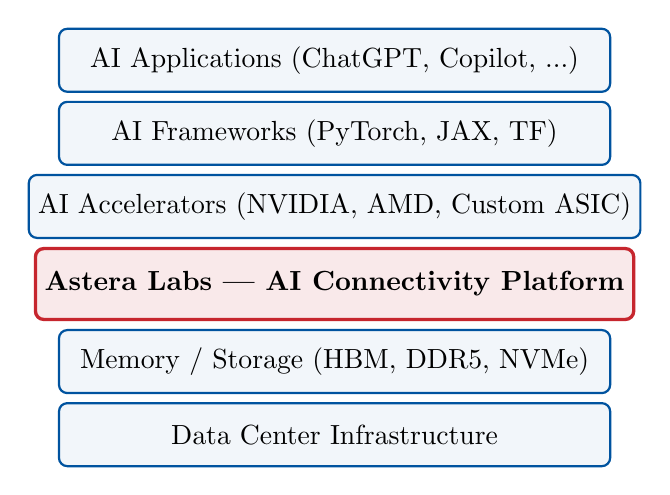
\begin{tikzpicture}[
    node distance=0.5cm,
    layer/.style={rectangle, draw=ieeeBlue, fill=ieeeBlue!5, thick,
                  minimum width=7cm, minimum height=0.8cm, align=center,
                  rounded corners=3pt},
    highlight/.style={rectangle, draw=ieeeRed, fill=ieeeRed!10, very thick,
                      minimum width=7cm, minimum height=0.9cm, align=center,
                      rounded corners=3pt}
  ]
    \node[layer] (APP) {AI Applications (ChatGPT, Copilot, ...)};
    \node[layer, below=0.1cm of APP] (FW) {AI Frameworks (PyTorch, JAX, TF)};
    \node[layer, below=0.1cm of FW] (GPU) {AI Accelerators (NVIDIA, AMD, Custom ASIC)};
    \node[highlight, below=0.1cm of GPU] (AST)
      {\textbf{Astera Labs — AI Connectivity Platform}};
    \node[layer, below=0.1cm of AST] (MEM) {Memory / Storage (HBM, DDR5, NVMe)};
    \node[layer, below=0.1cm of MEM] (INFRA) {Data Center Infrastructure};
  \end{tikzpicture}

  \vspace{-11pt}
  \begin{columns}[T]
    \begin{column}{0.55\textwidth}
      \begin{enumerate}
        \item 有\textbf{真实技术}和\textbf{正确战略}
        \item 先发优势窗口期：\textbf{2-3 年}
        \item COSMOS 是长期护城河的\textbf{关键变量}
        \item 核心 Paradox：NVIDIA 越封闭 $\leftrightarrow$ Astera 越有价值
      \end{enumerate}
    \end{column}
    \begin{column}{0.40\textwidth}
      \begin{exampleblock}{总体评级 (非投资建议)}
        \begin{itemize}
          \item 公司质量：\textbf{A-}
          \item 估值敏感性：高
          \item 竞争风险：\textbf{中等偏高}
        \end{itemize}
      \end{exampleblock}
    \end{column}
  \end{columns}
\end{frame}

% ============================================
\section*{结束}
% ============================================

\begin{frame}[plain]
  \centering
  \vfill
  {\huge\color{ieeeBlue} 谢谢！欢迎提问与讨论}

  \vspace{20pt}
  {\large 葛良晨}

  \vspace{8pt}
  {\normalsize 2026年5月21日}

  \vspace{20pt}
  {\small\color{darkGray} 数据来源：SEC EDGAR XBRL (CIK: 0001736297), Astera Labs 官网,\\
    SemiAnalysis, PCI-SIG, CXL Consortium 等公开资料}
  \vfill
\end{frame}

\end{document}
